\documentclass[12pt, a4paper]{article} 
 
\usepackage[utf8]{inputenc}
 

\usepackage[bottom = 8em]{geometry} % to change the page dimensions
\geometry{a4paper} % or letterpaper (US) or a5paper or....
 
\usepackage{graphicx} % support the \includegraphics command and options
\usepackage{grffile}
 
\usepackage{booktabs} % for much better looking tables
\usepackage{array} % for better arrays (eg matrices) in maths
\usepackage{float}
\usepackage{paralist} % very flexible & customisable lists (eg. enumerate/itemize, etc.)
\usepackage{verbatim} % adds environment for commenting out blocks of text & for better verbatim
\usepackage{subfig} % make it possible to include more than one captioned figure/table in a single float
% These packages are all incorporated in the memoir class to one degree or another...
 
 
 
\usepackage{amsmath, amssymb}% for mathematical symbols
\usepackage[colorlinks=true,linkcolor=black]{hyperref} % for hyperreferences with black color
%\usepackage[T1]{fontenc} % Uncomment for norwegian document
%\usepackage[norsk]{babel} %
 
%%% HEADERS & FOOTERS
\usepackage{fancyhdr} % This should be set AFTER setting up the page geometry
\pagestyle{fancy} % options: empty , plain , fancy
\renewcommand{\headrulewidth}{0pt} % customise the layout...
\lhead{}\chead{}\rhead{}
\lfoot{}\cfoot{\thepage}\rfoot{}

 
%%% SECTION TITLE APPEARANCE
\usepackage{sectsty}
\allsectionsfont{\sffamily\mdseries\upshape} % (See the fntguide.pdf for font help)
% (This matches ConTeXt defaults)
 
%%% ToC (table of contents) APPEARANCE
\usepackage[nottoc,notlof,notlot]{tocbibind} % Put the bibliography in the ToC
\usepackage[titles,subfigure]{tocloft} % Alter the style of the Table of Contents
\renewcommand{\cftsecfont}{\rmfamily\mdseries\upshape}
\renewcommand{\cftsecpagefont}{\rmfamily\mdseries\upshape} % No bold!
 
 
%%% END Article customizations
 
%%% The "real" document content comes below...
 
\title{Subsymbolic AI assignment 3}
\author{Eivind Hærum \& \ Hong-Dang Lam}
\date{\today} % Activate to display a given date or no date (if empty),
         % otherwise the current date is printed 
 
\begin{document}
\pagenumbering{gobble}
\maketitle
%\begin{abstract}
% 
%Abstract
% 
%\end{abstract}
\newpage

\tableofcontents
\pagenumbering{roman}
\newpage

\section{EA}

The EA from the previous assignment was reused for the most part, and expanded upon in regard to genotype, phenotype, fitness evaluator, mutation and crossover for this specific problem. 
The parameters used for finding good solutions are as follows:

\begin{figure}[H]
	\begin{center}
	\begin{tabular}{c|c|c}
		Population size & Adult Selection & Parent Selection \\
		\hline
		30 & Generational Mixing  & Tournament Selection(K=20,P=0.8) \\
		\hline
		\hline
		Crossover Rate & Mutation Rate & Mutation chance on each component\\
		\hline
		0.3 & 0.2 & Yes\\
	\end{tabular}
	\end{center}
\end{figure}

There are overall very little change in the fitness of the population when choosing other kinds of parent selection, or when altering the values of mutation rate and crossover rate. Thus we ended up with something that seems to work just as fine as many other combinations, but ultimately we chose this as it made a lot of sense. We did not include direct elitism in parent selection, but we did not find the need for that when using Tournament Selection.

\pagenumbering{arabic}

\section{Fitness}
The fitness function calculates how many cakes/food the agent have eaten and how many poisons it have eaten for each scene. The fitness evaluator gives points for each cake eaten, and punishes the "network" for each poison it obtains. These values are provided from each scene after a run with the proposed weights, and is calculated individually for the 5 scenes, summed up and finally divided by 5. Which makes the total score for the individual. The total score is whats compared to with the other individuals.
A mathematical formula for the fitness function is:
$$ \frac{\sum_{i=0}^{i =5}({\frac{foodEaten_i}{0.85 * totalFood_i} - \frac{poisonEaten_i}{totalPoison_i}})}{5} $$

The thought behind this equation is to punish eating poison, but also to give a slightly higher score for eating cake, thus the agent is encouraged to eat as much cake as possible in the allotted time and avoid eating poison. 

\section{ANN design}
We wanted to keep the ANN as simple as possible, that's why we decided to use direct mapping, meaning that there are 6 sensor inputs (3 for poison and 3 for food) and 3 output nodes. No hidden layers, although we did try to with a hidden layer of 3 nodes, but the result didn't vary as far as we could tell.
We decided to use the sigmoid function $$ \frac{1.0}
{(1+e^ {-\sum_{i = 0}^{n}{w_i * x_i}})} $$
as neuron activation, the step function works as well.  
$$
f(n) =
\begin{cases}
1, & \text{if} \sum_{i = 0}^{n}{w_i * x_i}>\text{threshold} \\
0, & \text{otherwise }
\end{cases}
$$

The outcoming of choosing this instead is very similar, but slightly worse.
The threshold we decided to use is 0.5, this was the first value we tried and it seems to work pretty good. As for weight range, the EA uses $[-1.0, 1.0]$. We tried to set the weight manually in the beginning and found out that we needed negative weights. The range from -1 to 1 seems sufficient. This is also due to the fact that the neurons will fire at the range $[0,1.0]$, and the only way to negate a fired neuron (in the sense of punishing its values, not ignoring it) is to set the connecting weight to a negative value.

\section{Differences in dynamic vs static}
For a dynamic run we got:\\
\begin{figure}[H]
	\begin{center}
	\begin{tabular}{l| c|c|c|c|c}
	Run number: &  1&2 &3 &4 &5 \\ \hline
cakes eaten: &$ \frac{26}{32} $ &$ \frac{25}{31} $ &$ \frac{23}{30} $ &$ \frac{22}{30} $ &$ \frac{25}{33} $ \\ \hline
poison eaten: &$ \frac{0}{14} $ &$ \frac{0}{14} $ &$ \frac{0}{14} $ &$ \frac{0}{14} $ &$ \frac{0}{19} $ \\ 
	\end{tabular}
	\end{center}
\end{figure}
The total for this becomes: $ \frac{121}{156} $ cakes and $ \frac{0}{75} $ poisons.  
\begin{figure}[H]
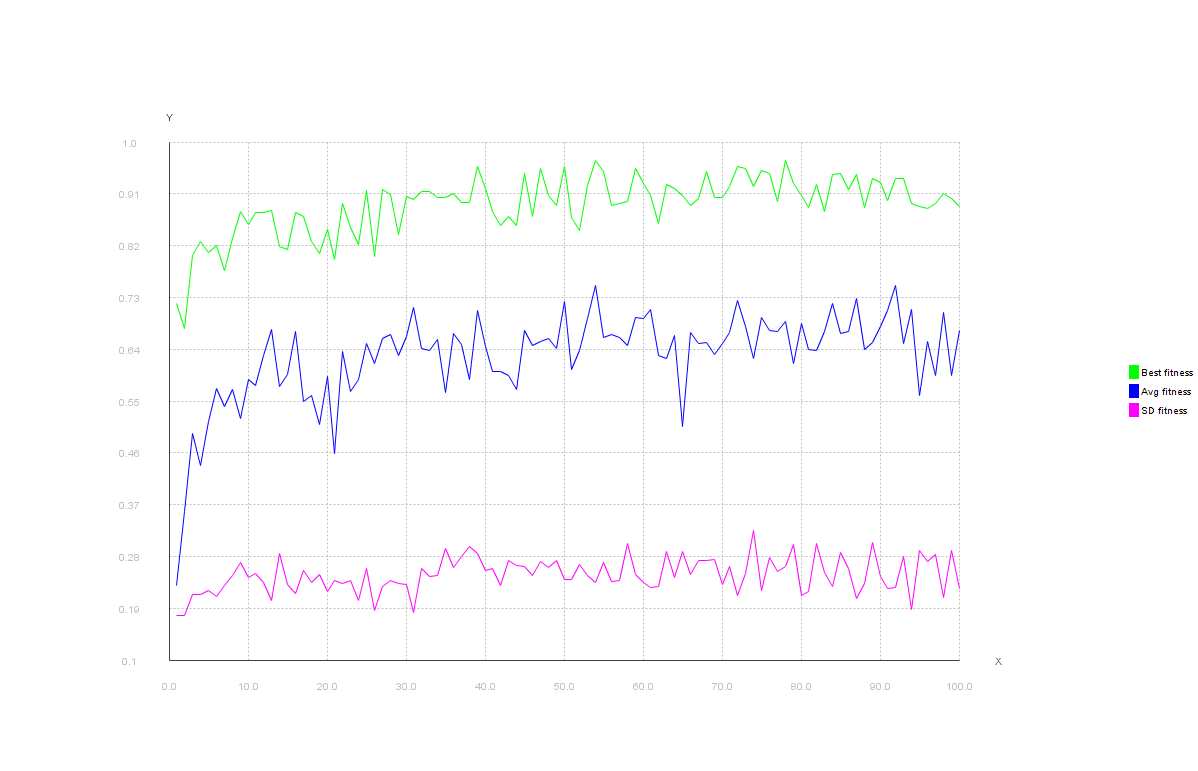
\includegraphics[width=0.9\linewidth]{flatlandtrue}
\caption{Graph of EA runs on a dynamic set}
\end{figure}

For a static run we got:\\
\begin{figure}[H]
	\begin{center}
	\begin{tabular}{l| c|c|c|c|c}
	Run number: &  1&2 &3 &4 &5 \\ \hline
cakes eaten: &$ \frac{20}{29} $ &$ \frac{22}{30} $ &$ \frac{22}{33} $ &$ \frac{22}{30} $ &$ \frac{21}{30} $ \\ \hline
poison eaten: &$ \frac{0}{15} $ &$ \frac{0}{10} $ &$ \frac{0}{18} $ &$ \frac{0}{17} $ &$ \frac{1}{17} $ \\ 
	\end{tabular}
	\end{center}
\end{figure}
The total for this becomes: $ \frac{107}{152} $ cakes and $ \frac{1}{77} $ poisons.
\begin{figure}[H]
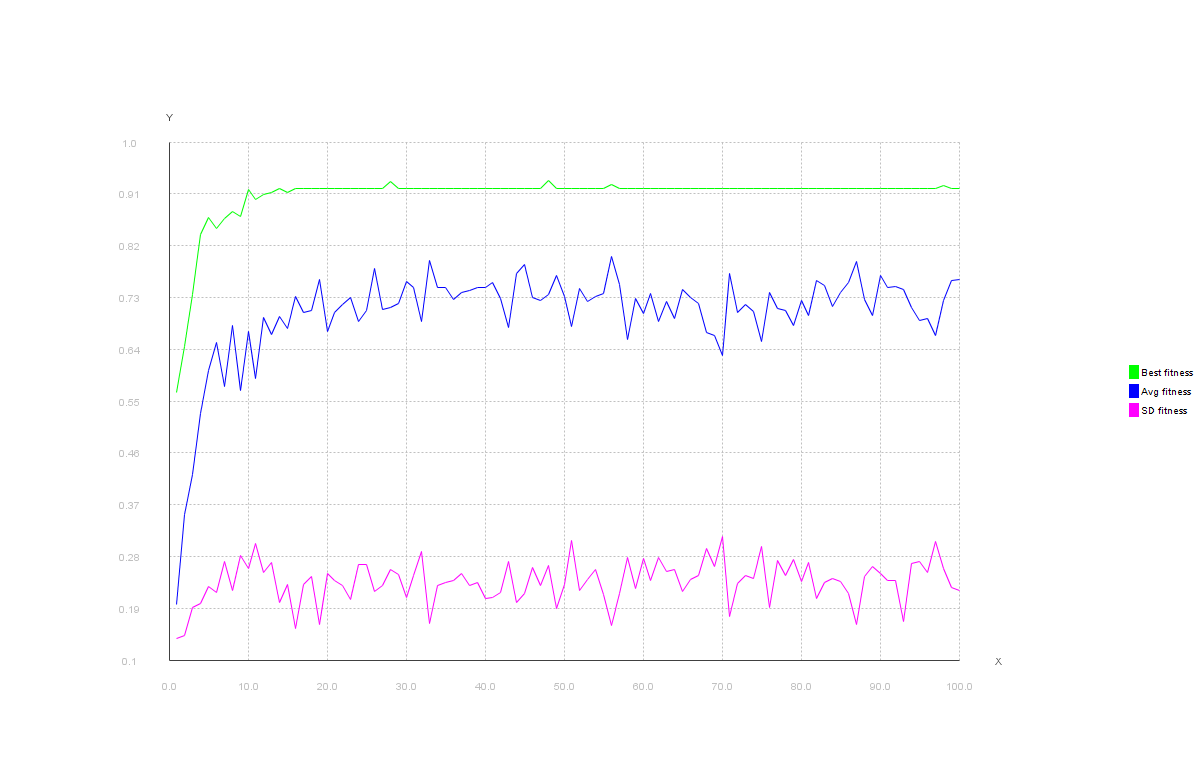
\includegraphics[width=0.9\linewidth]{flatlandfalse}
\caption{Graph of EA runs on a static set}
\end{figure}

The dynamic run seems to give better results, this is likely due to the change in scenes for each generation. Which means that the individuals have a larger set of training examples they can explore and learn from, thus tactics that may yield good short time results are weeded out in the long haul.

\section{demo of static and dynamic}
Refer to the demo for this.

Following below are some screen dumps of the gui.
\begin{figure}[H]
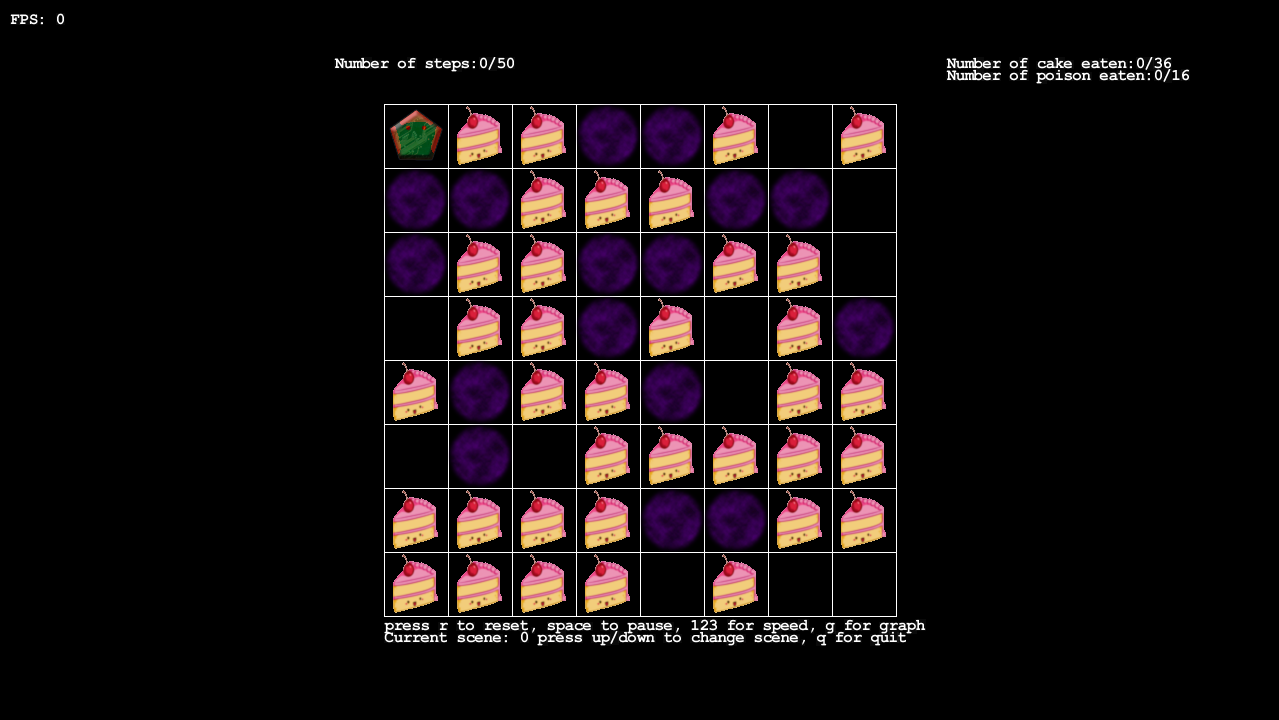
\includegraphics[width=\linewidth]{flatland_dump}
\caption{A run before the agent has initated}
\end{figure}
\begin{figure}[H]
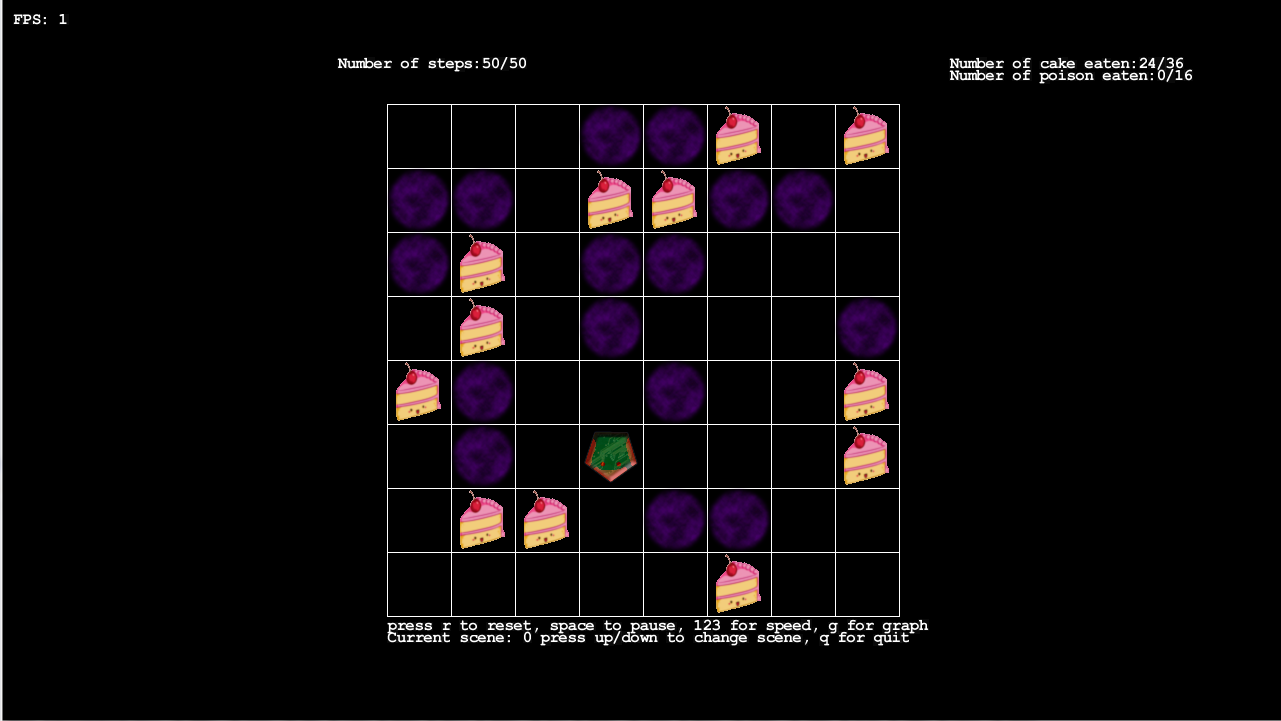
\includegraphics[width=\linewidth]{flatland_dump_complete}
\caption{A run after the agent has completed its job}
\end{figure}
\end{document}
